\documentclass[11pt]{article}

%Both greek and english language support
\usepackage[greek,english]{babel}
\usepackage[utf8]{inputenc}
\usepackage{alphabeta}

% For \includegraphics
\usepackage{graphicx}   
\usepackage[space]{grffile}

\usepackage{amsmath}
\usepackage{amssymb}
\usepackage{float}

\usepackage[makeroom]{cancel}
\usepackage[colorinlistoftodos]{todonotes}

% For hyper links
\usepackage[unicode]{hyperref}

%Diagonal line on Tables\documentclass[11pt]{article}
\usepackage{diagbox}

%Multiple rows in tables
\usepackage{multirow}

% %----------------------------- MATLAB -----------------------------
\usepackage[T1]{fontenc}
% \usepackage{bigfoot} % to allow verbatim in footnote
\usepackage[numbered,framed]{matlab-prettifier}

\lstset{
  style              = Matlab-editor,
  basicstyle         = \mlttfamily,
  escapechar         = ",
  mlshowsectionrules = true,
}
\let\ph\mlplaceholder % shorter macro
\lstMakeShortInline"

% % In order to use Matlab code just use this 
% \begin{lstlisting}[caption = {Title}]
%   code
% \end{lstlisting}
% %----------------------------- MATLAB -----------------------------

% Page margins 
\usepackage{geometry}
 \geometry{
 a4paper,
 total={170mm,257mm},
 left=20mm,
 top=20mm,
 }

\DeclareUnicodeCharacter{2212}{-}   %Negative exponential


\begin{document}
    %--------------------------------------------------------------------------------------------
    % Title Page
    \begin{titlepage}
        \center
        %----------------------------------------------------------------------------------------
        %	HEADING SECTIONS
        \textsc{\LARGE Technical University of Crete}\\[2cm] 
        \Large Τηλεπικοινωνιακά Συστήματα Ι\\[1cm] 
        
        \rule{\linewidth}{0.5mm} \\[0.5cm]
            { \huge \bfseries Άσκηση 3}\\[0.5cm]
        \rule{\linewidth}{0.5mm} \\[2.5cm]
        
        \begin{minipage}{0.4\textwidth}
            \begin{flushleft} \large
                \emph{Author:}\\
                    Σπυριδάκης Χρήστος
            \end{flushleft}
        \end{minipage}
        ~
        \begin{minipage}{0.4\textwidth}
            \begin{flushright} \large
                \emph{ΑΜ:} 2014030022
            \end{flushright}
        \end{minipage}\\[4cm]
        
        {\large January 9, 2019}\\[2cm] 
        %----------------------------------------------------------------------------------------
        %	LOGO
        
\includegraphics[scale=0.5]{TUC.png} 
        \vfill
    \end{titlepage}



    % %-------------------------------------
    % %   A. subsection
    % \subsection*{A. }
    % Εισαγωγή: 
    
    % \begin{figure}[H]
    %     \centering
    %     \includegraphics[scale=0.5, width=0.8\textwidth]{photos/} \\
    %     \caption{}
    % \end{figure}
    
    % \begin{lstlisting}[caption = {}]
    %     code
    % \end{lstlisting}
    % \par \noindent
    % Συμπεράσματα:
    
    

    % \par \noindent
    %-------------------------------------------------------------------------
    %   Eisagwgi
    \section*{Εισαγωγή}
    Για την διευκόλυνση της υλοποίησης είναι καλό να σημειωθεί ότι το κάθε μέρος υλοποιήθηκε σε διαφορετικό script, αυτό είχε τα θετικά του, στο να είναι περισσότερο διακριτός ο κώδικας για ανάπτυξη και αποσφαλμάτωση, αλλά χρειάστηκε να ξανά δημιουργηθούν σήματα που είχαν δημιουργηθεί σε προηγούμενα ερωτήματα. Δεν επηρεάζονται κάπως τα αποτελέσματα απλά είναι μία διευκρίνηση σχετικά με την δομή που δόθηκε στον κώδικα. 
    \par \noindent
    Επίσης παρατηρήθηκε ότι κατά την διάρκεια της άσκησης είναι πολλά πράγματα τα οποία μοιάζουν μεταξύ των ζητουμένων. Ακολουθήθηκε λοιπόν μία τακτική δομημένου προγραμματισμού με χρήση συναρτήσεων, προκειμένου ενέργειες που ζητούνται από περισσότερο του ενός σημεία, να μην επαναλαμβάνονται από το μηδέν. Για αυτό το λόγο υπάρχουν πολλαπλά βοηθητικά αρχεία τα οποία δημιουργήθηκαν. Σε κάθε ενότητα όπως χρειάζεται θα εισαγάγεται η λειτουργικότητα της κάθε συνάρτησης που περιέχεται σε ένα αρχείο και στην συνέχεια θα δείχνεται μόνο ο τρόπος κλήσης της. Τα αρχεία τα οποία υπάρχουν συνολικά για την ολοκληρωμένη εκτέλεση της άσκησης είναι τα εξής: \emph{\texttt{srrc\_pulses.m}} , \emph{\texttt{bits\_to\_4\_PAM.m}} , \emph{\texttt{detect\_4\_PAM.m}} , \emph{\texttt{PAM\_4\_to\_bits.m}} , \emph{\texttt{fourier\_transform.m}} ,  \emph{\texttt{display\_waveform\_periodogram.m}} , \emph{\texttt{periodogram.m}} , \emph{\texttt{part\_a.m}} , \emph{\texttt{part\_b.m}}.
    \par \noindent
    Να αναφερθεί ότι στους ενδιάμεσους κώδικες (για το κάθε ερώτημα) εμφανίζεται ΜΟΝΟ το κομμάτι υπολογισμού του ερωτήματος, δεν εμφανίζονται δηλαδή κατά κύριο λόγω κομμάτια κώδικα σχετικά με την δημιουργία των figure ή τις έξτρα πληροφορίες για αυτά - αν δεν είναι σημαντικό - όπως επίσης και κάποια από τα σχόλια για εξοικονόμηση χώρου. Γενικά έχει ελαφρώς αλλαχθεί ο κώδικας που παρουσιάζεται σε κάθε ερώτηση ώστε να κρατηθούν μόνο τα σημαντικά σημεία. Στο τέλος της αναφοράς υπάρχει ολόκληρος ο κώδικας για έλεγχο και αυτών των σημείων.
    \par \noindent
    Τέλος, αν λόγω της εκτύπωσης σε χαρτί δεν είναι εμφανές σε ικανοποιητικό βαθμό κάποιο από τα figures μπορούν να βρεθούν όλα τα μέρη του project στο παρακάτω repository όπου υπάρχουν και screenshot αυτών, που φαίνονται με καλύτερη ανάλυση: \url{https://github.com/CSpyridakis/CommSys}

    %-------------------------------------------------------------------------
    %   A section
    \section*{Ερώτημα Α} 
    
    %-------------------------------------
    %   A.1 subsection
    \subsection*{A.1 Create random bits}
    Πρώτο ζητούμενο της συγκεκριμένης άσκησης είναι να δημιουργηθεί μία δυαδική ακολουθία με 4Ν ισοπίθανα bits. 
    Για να γίνει αυτό, χρησιμοποιήσαμε τον κώδικα που εμφανίζεται στο listing 1 και είναι όπως έχει πραγματοποιηθεί και στις προηγούμενες ασκήσεις για αυτό δεν γίνεται περαιτέρω ανάλυση. 
    Το μόνο που πρέπει να σημειωθεί είναι ότι επιλέχθηκε ως $Ν=200$. 
    Συνεπώς θα δημιουργούνταν 800 τυχαία bits.
    
   \begin{lstlisting}[caption = {A.1 Create random bits}]
% A.1
N = 200;                                % Random bits E.g. 
bit_seq = (sign(randn(4*N, 1)) + 1)/2;  % 0 1 1 0 0 1 1 1. . .
    \end{lstlisting}
    
    %-------------------------------------
    %   A.2 subsection
    \subsection*{A.2 Bits to 4-PAM} 
    Αφού κάναμε το Α1 έπρεπε να συντάξουμε συνάρτηση \emph{\texttt{bits\_to\_4\_PAM(bit\_seq, A)}} παρόμοια με αυτή που κάναμε στο δεύτερο project με την διαφορά ότι θα έπρεπε σε αυτή να χρησιμοποιήσουμε κώδικα Gray στην αναπαράσταση bit σε σύμβολα 4-PAM. 
    Αυτό που μας βοηθάει η κωδικοποίηση Gray είναι ότι στην περίπτωση όπου έχουμε σφάλμα στην μετάδοση ενός συμβόλου και τυγχάνει να πάρουμε ένα γειτονικό σύμβολο αντί αυτού (κάτι που κατά πάσα πιθανότητα αυτό θα συμβεί όταν έχουμε σωστό σχεδιασμό), επειδή το ένα σύμβολο από το άλλο διαφέρουν μόνο κατά 1 bit έτσι και το σφάλμα σε επίπεδο bit θα είναι σε αυτήν την περίπτωση μόνο ένα.

    \newpage
    
    \begin{lstlisting}[caption = {A.2 \texttt{bits\_to\_4\_PAM(bit\_seq, A)}}]
function [ X ] = bits_to_4_PAM(bit_seq, A)
    k=1;
    X=zeros(1,length(bit_seq)/2);
    for i=1:2:length(bit_seq)
        if(bit_seq(i)==0 && bit_seq(i+1)==0)        % 00 -> +3
            X(k) = 3*A;
        elseif(bit_seq(i)==0 && bit_seq(i+1)==1)    % 01 -> +1
            X(k) = 1*A;
        elseif(bit_seq(i)==1 && bit_seq(i+1)==1)    % 11 -> -1
            X(k) = -1*A;
        elseif(bit_seq(i)==1 && bit_seq(i+1)==0)    % 10 -> -3
            X(k) = -3*A;
        end
        k=k+1;
    end
end
    \end{lstlisting}
    
    \par \noindent
    Αφού είχαμε δημιουργήσει την συνάρτηση αυτή (η οποία έγινε με χρήση απλών συνθηκών ελέγχου), το μόνο που χρειαζόταν ήταν στο κύριο πρόγραμμα να την καλέσουμε για $Α=1$ ώστε να μετατρέψουμε τα τυχαία bits που δημιουργήσαμε σε σύμβολα. 
    Αφού έχουμε επιλέξει $Ν=200$ συνεπώς έχουμε στο bit\_seq μέγεθος 800bits και επειδή δύο bits μας δίνουν ένα σύμβολο 4-PAM, θα έχουμε 400 σύμβολα στο Xn.
    
    \begin{lstlisting}[caption = {A.2 \texttt{Convert bits to symbols}}]
% A.2
A = 1;                          % Bits to 4 Pam E.g
Xn = bits_to_4_PAM(bit_seq, A);  % +1 -3 -1 -1 +3 . 
    \end{lstlisting}
    
    %-------------------------------------
    %   A3 subsection
    \subsection*{A.3 \{$X_{I,n}$\} and \{$X_{Q,n}$\} }
    Έχοντας κάνει τα παραπάνω `σπάσαμε' την ακολουθία συμβόλων σε δύο ξεχωριστές. 
    Η πρώτη είναι η $X_{I,n}$ για $n=1, ..., N$ για τα 2Ν πρώτα bits. 
    Ενώ η δεύτερη $X_{Q,n}$ για $n=1, ..., N$ για τα 2Ν τελευταία bits. 
    Συνεπώς στην κάθε μία υπάρχουν 200 σύμβολα.
    
    
    \begin{lstlisting}[caption = {A.3 \texttt{Split Symbols}}]
% A.3
XI_n = Xn(1:N);                    % In Phase Symbols
XQ_n = Xn(N+1:2*N);                % Quadrature Symbols
    \end{lstlisting}
    
    
     \begin{figure}[H]
        \centering
        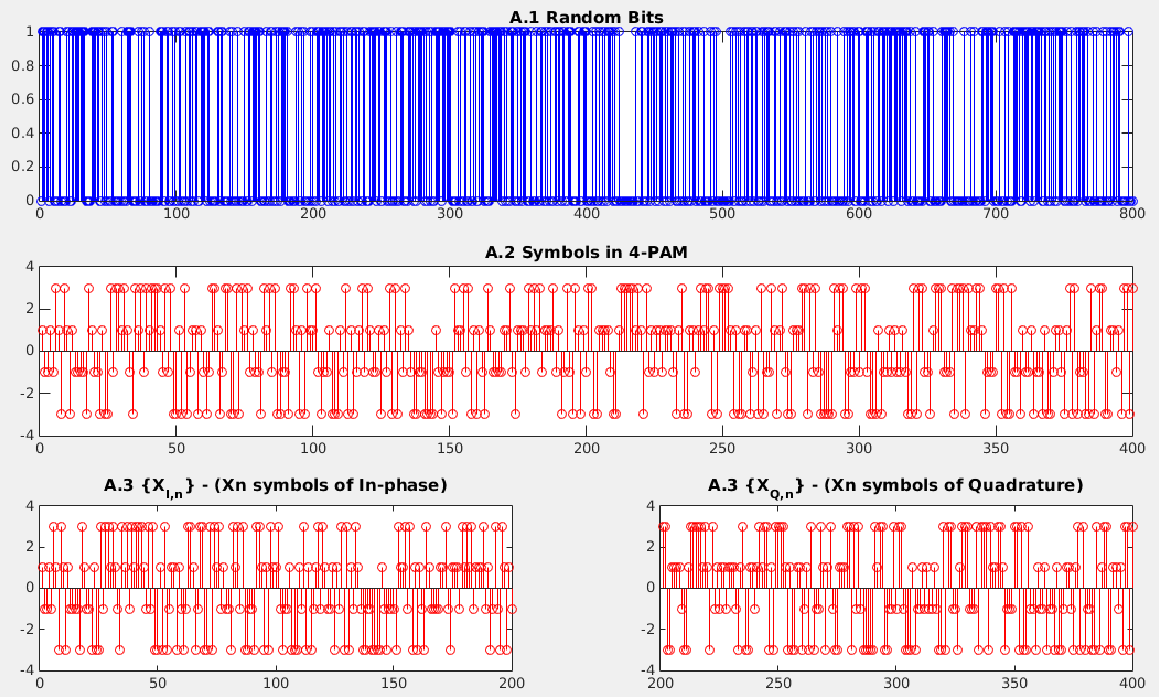
\includegraphics[scale=0.5, width=0.9\textwidth]{img/A1_A3.png} \\
        \caption{\texttt{Random Bits, 4-PAM Symbols and Inphase/Quadrature Symbols}}
    \end{figure}
    
     %-------------------------------------
    %   A.4 subsection
    \subsection*{A.4 $X_I(t)$ and $X_Q(t)$}
    
    Σε αυτό το σημείο αφού είχαμε τις δύο ακολουθίες συμβόλων - $X_{I,n}$ και $X_{Q,n}$ - χρειάστηκε να τις περάσουμε από τα SRRC φίλτρα μορφοποίησης.
    Για τα φίλτρα χρησιμοποιήθηκε $T=0.01$ sec, $over = 10$, $T_s = \frac{T}{over}$ ενώ για το Α και α δόθηκαν οι τιμές που δοκιμάστηκαν στο δεύτερο project δηλαδή $Α=4$ και $a=0.5$. 
    Στο listing 5 εμφανίζεται ο τρόπος με τον οποίο περνάμε τις δύο συμβολοσειρές από τα φίλτρα. 
    Ουσιαστικά είναι με τον ίδιο τρόπο που ήδη έχει παρουσιαστεί στα προηγούμενα project, συνεπώς δεν ξανά αναλύεται. 
    Επίσης να αναφερθεί ότι το $Nf=2048$ κατά όλη την διάρκεια της άσκησης.
    
    \begin{lstlisting}[caption = {A.4 \texttt{Calculate $X_I(t)$ and $X_Q(t)$}}]
% A.4
T = 0.01 ; over = 10 ; Ts = T/over ; A_s = 4 ; a = 0.5;
Nf = 2048 ; Fs = 1/Ts ; F = [-Fs/2 : Fs/Nf : Fs/2-Fs/Nf]; % Frequency vector

% Phi
[phi_t t_phi] = srrc_pulse(T, Ts, A_s, a);

% Create upsampled X_delta signals and using it calculate conv
XI_d = 1/Ts * upsample(XI_n, over) ; XI_t = conv(XI_d, phi_t).*Ts ;
XQ_d = 1/Ts * upsample(XQ_n, over) ; XQ_t = conv(XQ_d, phi_t).*Ts ;
td = [0 : Ts : (N*over-1)*Ts ]; t_Xt = [td(1) + t_phi(1) : Ts : td(end) + t_phi(end)];

display_waveform_periodogram('A.4', 'X_i(t)', XI_t, 'X_q(t)', XQ_t, t_Xt,t_Xt, Ts, Nf)
    \end{lstlisting}
    
    \par \noindent
    Στο listing 5 παρουσιάζεται η συνάρτηση display\_waveform\_periodogram(). Ουσιαστικά ο ρόλος της συγκεκριμένης συνάρτησης είναι να εμφανίζει 
    την κυμματοφορφή/κυμματομορφές που της δίνονται ως είσοδο, να υπολογίζει το/τα περιοδόγραμμα τους και να εμφανίζει και αυτά. 
    Δεν δίνεται περισσότερη ανάλυση εδώ καθώς είναι κυρίως εντολές σχετικά με εμφάνιση (figure, plot, etc...) και η χρήση της custom συνάρτησης periodogram() που δημιουργήθηκε και αναλύθηκε στο δεύτερο project και σκοπό έχει να υπολογίζει το περιοδόγραμμα ενός σήματος. 
    Παρόλα αυτά δίνεται στο τέλος η υλοποίηση της.
    
     \begin{figure}[H]
        \centering
        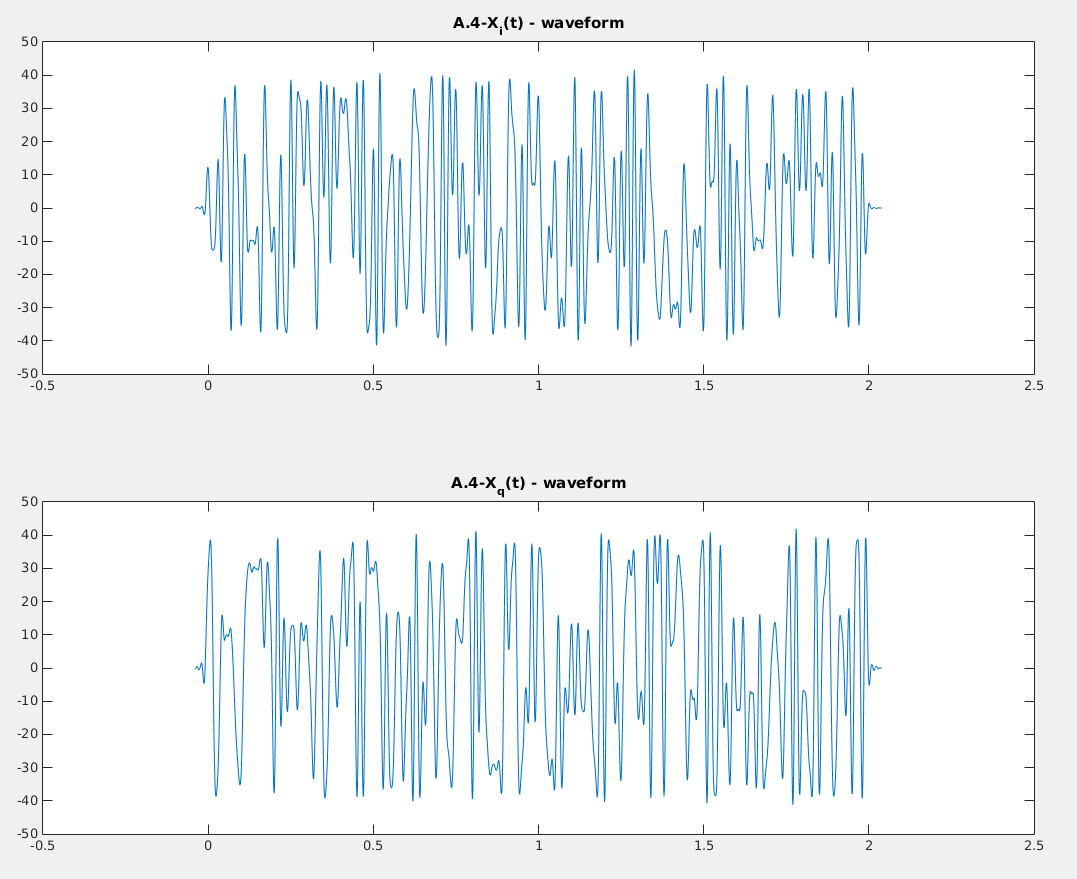
\includegraphics[scale=0.5, width=0.8\textwidth]{img/A4_wave.png} \\
        \caption{\texttt{$X_I(t)$ and $X_Q(t)$ waveforms}}
    \end{figure}
    
    \begin{figure}[H]
        \centering
        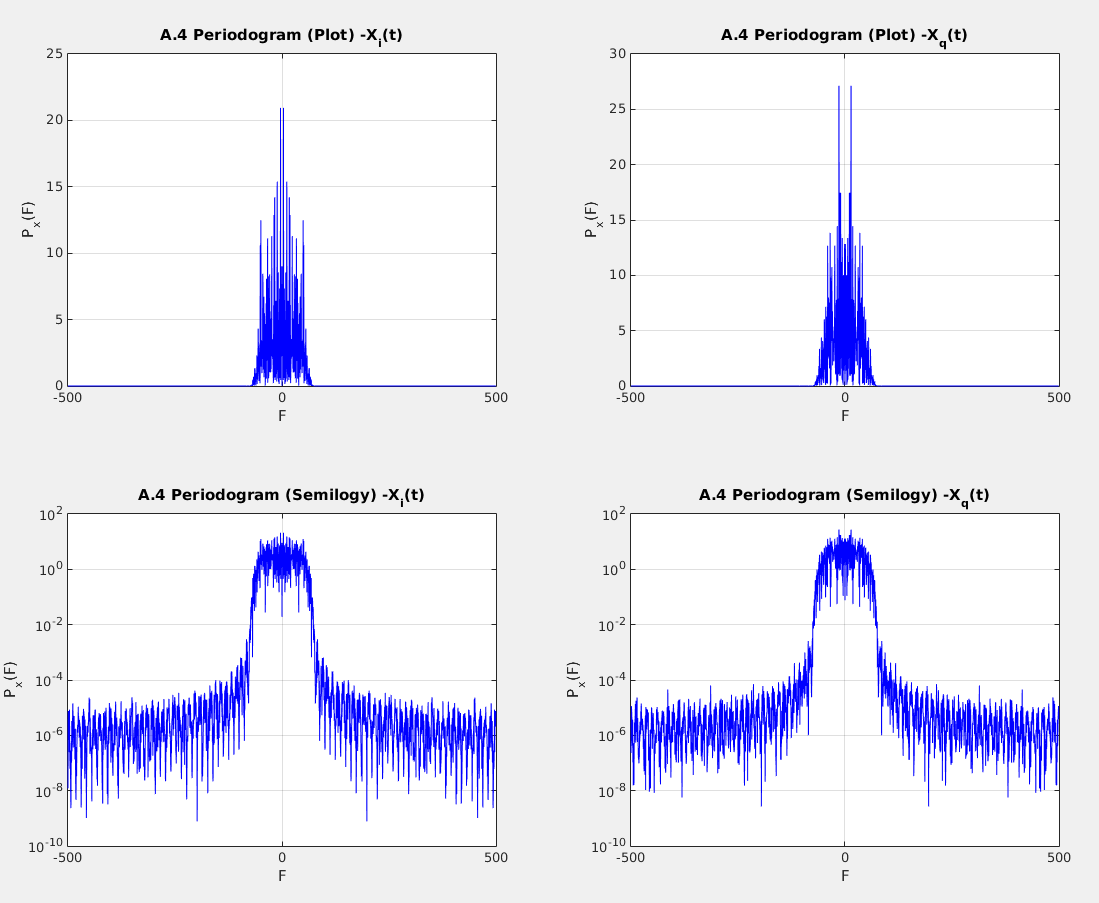
\includegraphics[scale=0.5, width=0.8\textwidth]{img/A4_Period.png} \\
        \caption{\texttt{$X_I(t)$ and $X_Q(t)$ periodograms}}
    \end{figure}
    
     %-------------------------------------
    %   A.5 subsection
    \subsection*{A.5 $X_I^{mod}(t)$ and $X_Q^{mod}(t)$}
    Έπειτα, αυτό που ζητήθηκε ήταν να πολλαπλασιάσουμε τις κυμματομορφές $X_I(t)$ και $X_Q(t)$ με τους αντίστοιχους φορείς για $F_o=200Hz$ (όπως διευκρινίστηκε στην διόρθωση μέσω e-mail) ώστε να δημιουργήσουμε τις κυμματομορφές $X_I^{mod}(t)$ και $X_Q^{mod}(t)$. 
    Ουσιαστικά έπρεπε να ακολουθήσουμε τους μαθηματικούς τύπους της εκφώνησης ώστε να κάνουμε την διαμόρφωση, για την δημιουργία των δύο συνιστωσών της εισόδου του καναλιού.
    
    \begin{lstlisting}[caption = {A.5 \texttt{Calculate $X_I^{mod}(t)$ and $X_Q^{mod}(t)$}}]
% A.5
Fo = 200;
XI_mod =  2 * XI_t .* cos(2*pi*Fo*t_Xt);
XQ_mod = -2 * XQ_t .* sin(2*pi*Fo*t_Xt);
display_waveform_periodogram('A.5', 'X_i^{mod}', XI_mod, 'X_q^{mod}', XQ_mod, t_Xt, t_Xt, Ts, Nf)
    \end{lstlisting}
    
    \begin{figure}[H]
        \centering
        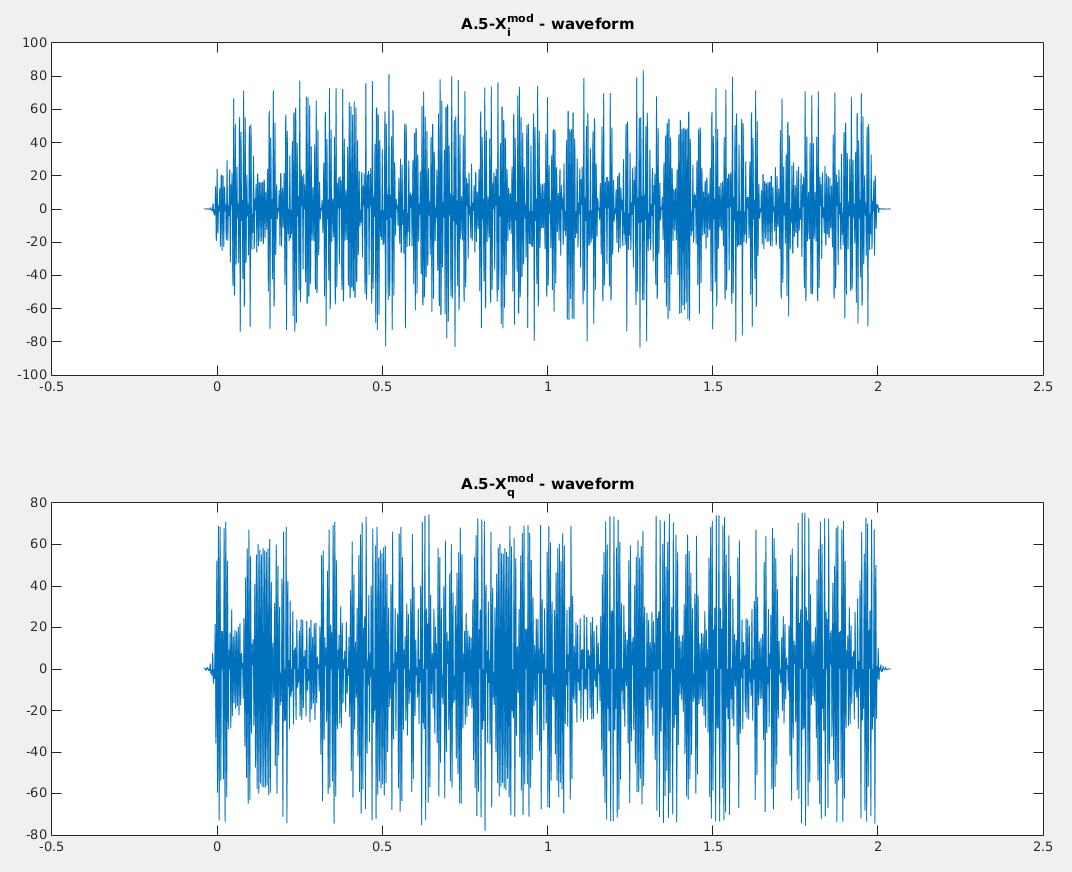
\includegraphics[scale=0.5, width=0.9\textwidth]{img/A5_mod_wave.png} \\
        \caption{\texttt{$X_I^{mod}(t)$ and $X_Q^{mod}(t)$ waveforms}}
    \end{figure}
    
    \begin{figure}[H]
        \centering
        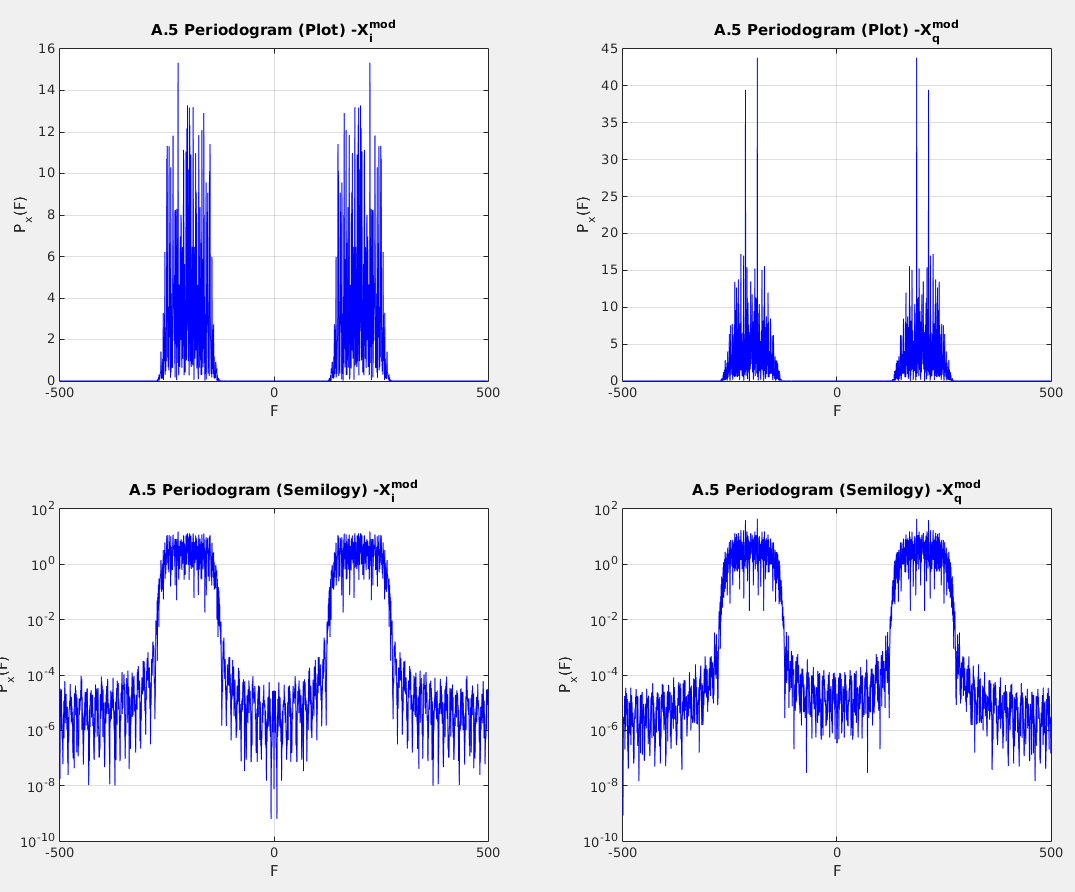
\includegraphics[scale=0.5, width=0.9\textwidth]{img/A5_mod_period.png} \\
        \caption{\texttt{$X_I^{mod}(t)$ and $X_Q^{mod}(t)$ periodograms}}
    \end{figure}
    
    \par \noindent
    Αυτά που μπορούμε να παρατηρήσουμε είναι, αρχικά οι κυμματοφορφές ότι έχουν μεγαλύτερο πλάτος και μεγαλύτερη συχνότητα λόγω του πολλαπλασιασμού, ενώ πιο συγκεκριμένα βλέπουμε τα περιοδογράμματα ότι έχουν μετακινηθεί γύρω από την συχνότητα μετάδοσης (Fo=200Hz) και είναι συμμετρικά ως προς το 0.
    
     %-------------------------------------
    %   A.6 subsection
    \subsection*{A.6  $X^{mod}(t)$}
    Στην συνέχεια έπρεπε απλά να συνδιάσουμε τις δύο παραπάνω συνιστώσες για να δημιουργήσουμε την είσοδο του καναλιού, δηλαδή το σήμα $X^{mod}(t)$ όπως το ονομάζουμε. 
    Αυτό το καταφέρνουμε με το να αθροίσουμε το Inphase και το Quadrature, ενώ παρακάτω έχουμε τα ζητούμενα figures. 
    
    
    \begin{lstlisting}[caption = {A.6 \texttt{Calculate $X^{mod}(t)$}}]
% A.6
t_X_mod = t_Xt;
X_mod = XI_mod + XQ_mod;
display_waveform_periodogram('A.6', ' X_{mod} = X_i^{mod} + X_q^{mod} - Plot', X_mod, '', [], t_X_mod, [], Ts, Nf)
    \end{lstlisting}
    
    \begin{figure}[H]
        \centering
        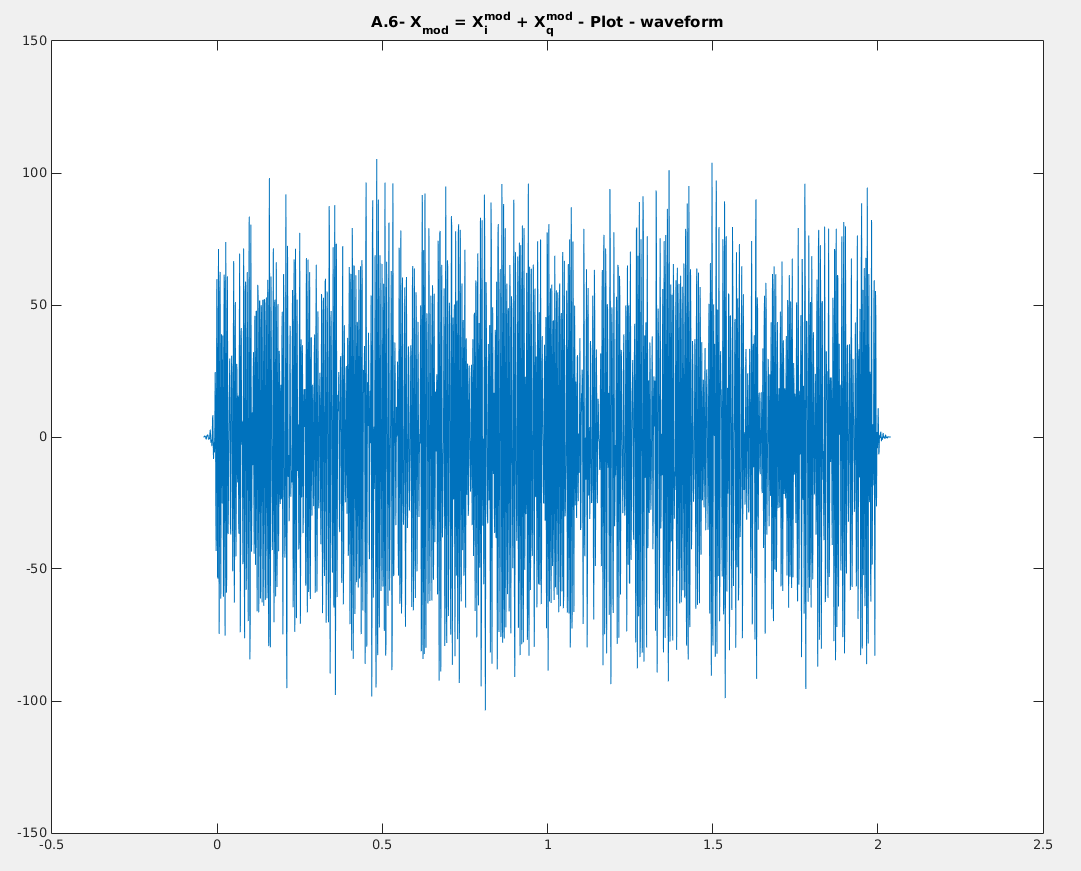
\includegraphics[scale=0.5, width=0.8\textwidth]{img/A6_mod_wave.png} \\
        \caption{\texttt{$X^{mod}(t)$ waveform}}
    \end{figure}
    
    \begin{figure}[H]
        \centering
        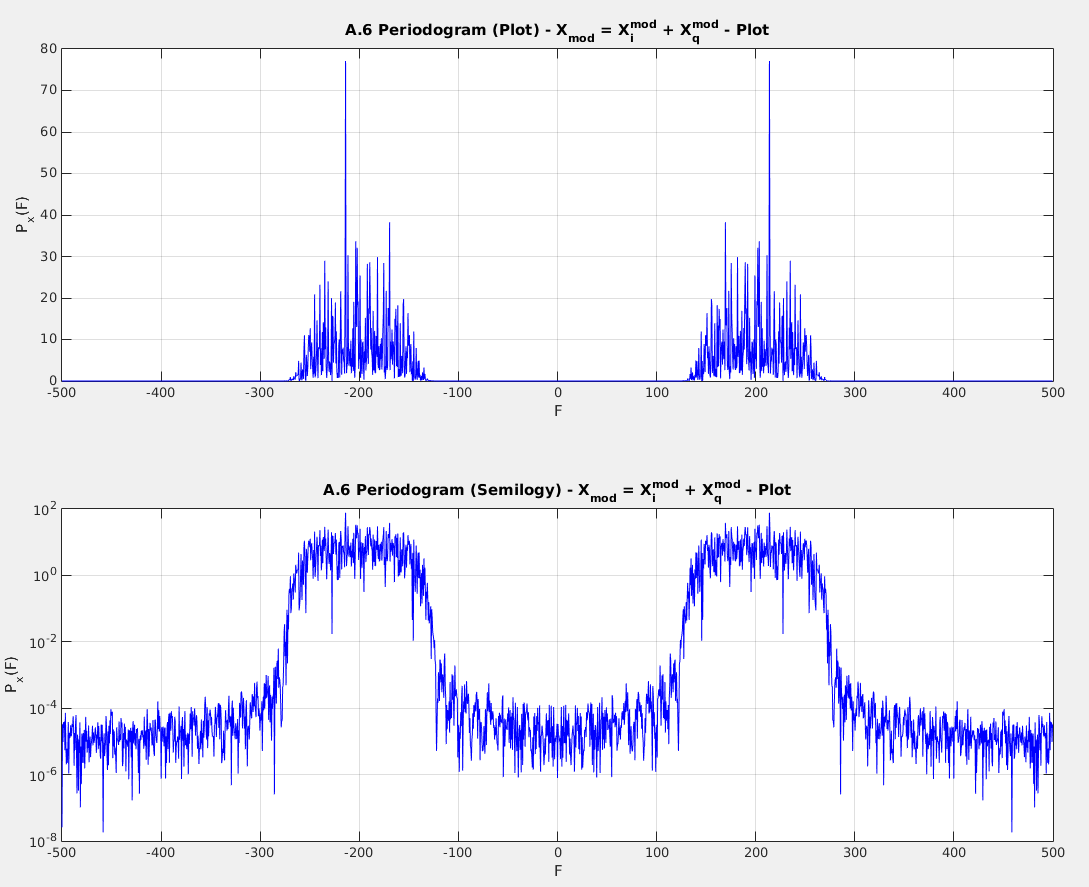
\includegraphics[scale=0.5, width=0.8\textwidth]{img/A6_mod_period.png} \\
        \caption{\texttt{$X^{mod}(t)$ periodogram}}
    \end{figure}
    
    \newpage \par \noindent
    Αυτό που μπορούμε να παρατηρήσουμε σε αυτήν την περίπτωση είναι ότι το φάσμα συνεχίζει να είναι γύρω από την συχνότητα μετάδοσης Fo και συμμετρικό ως προς το 0, με μόνη διαφορά ότι έχει αυξηθεί το πλάτος εξαιτίας της άθροισης.
    
    %-------------------------------------
    %   A.7 subsection
    \subsection*{A.7 Ιδανικό κανάλι}
    Αν είχαμε ιδανικό κανάλι, αυτό θα σήμαινε ότι δεν θα υπήρχε καμία αλλοίωσή στο σήμα κατά την μεταφορά. 
    Δηλαδή δεν θα υπήρχε κάποια μεταβολή στο πλάτος ή χρονική μετατόπιση κατά την μεταφορά του σήματος από την έξοδο του πομπό στην είσοδο του δέκτη.

    %-------------------------------------
    %   A.8 subsection
    \subsection*{A.8 Gaussian White Noise}
    Αντίθετα με το ιδανικό κανάλι που σε ελάχιστες περιπτώσεις στην πραγματικότητα μπορούμε να το προσεγγίσουμε, πιο συχνό είναι να υπάρχει θόρυβος σε αυτό.
    Συνεπώς σε αυτό το ερώτημα δημιουργήσαμε White Gaussian Noise (WGN) με την διασπορά που δίνεται στην εκφώνηση της άσκησης με $SNR_{dB}=10$ και το προσθέσαμε στην έξοδο του καναλιού.
    
    \begin{lstlisting}[caption = {A.8 \texttt{}}]
% A.8
SNR = 10;
var_n = (10*A^2)/(Ts*(10^(SNR/10)));
WGN = sqrt(var_n)*randn(1, length(X_mod));
ch_sig = X_mod + WGN;
    \end{lstlisting}
    
    %-------------------------------------
    %   A.9 subsection
    \subsection*{A.9 Received signals}
    Πλέον στην είσοδο του δέκτη είχαμε μία ενθόρυβη κυμματοφορφή, μέσα στην οποία περιεχόταν η πληροφορία που θέλαμε να μεταδώσουμε αρχικά.
    Πρώτο βήμα λοιπόν για την ανάκτηση της, ήταν να την διακλαδώσουμε και να την πολλαπλασιάσουμε με τους αντίστοιχους φορείς $cos(2 \pi Fo t)$ και $-sin(2 \pi Fo t)$.
    Αυτό που θέλουμε να επιτύχουμε ουσιαστικά είναι να αποδιαμορφώσουμε το σήμα που έχουμε εκλάβει. 
    
    \begin{lstlisting}[caption = {A.9 \texttt{}}]
% A.9
ch_sig_I = ch_sig.*cos(2*pi*Fo*t_X_mod);
ch_sig_Q = ch_sig.*(-1*sin(2*pi*Fo*t_X_mod));
display_waveform_periodogram('A.9', 'Received I', ch_sig_I, 'Received Q', ch_sig_Q, t_X_mod, t_X_mod, Ts, Nf)
    \end{lstlisting}
    
    \begin{figure}[H]
        \centering
        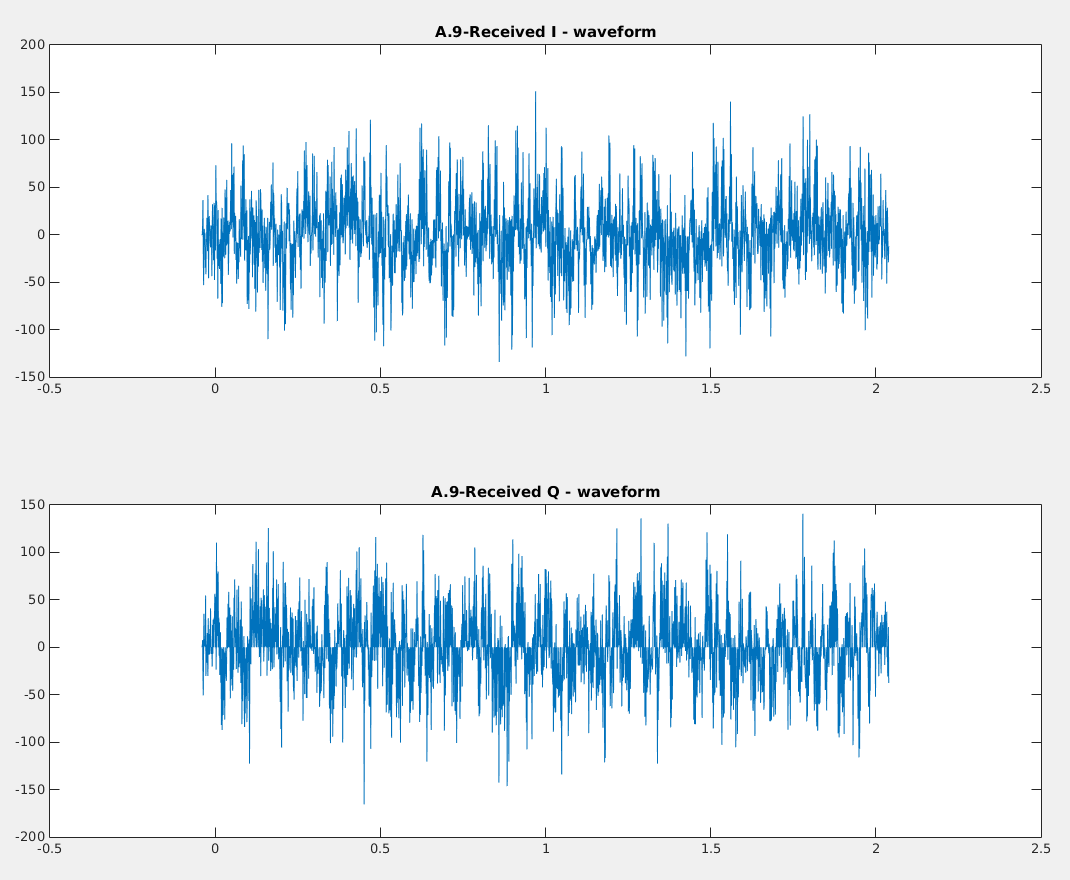
\includegraphics[scale=0.5, width=0.8\textwidth]{img/A9_rec_wave.png} \\
        \caption{\texttt{Received signals waveforms}}
    \end{figure}
    
    \begin{figure}[H]
        \centering
        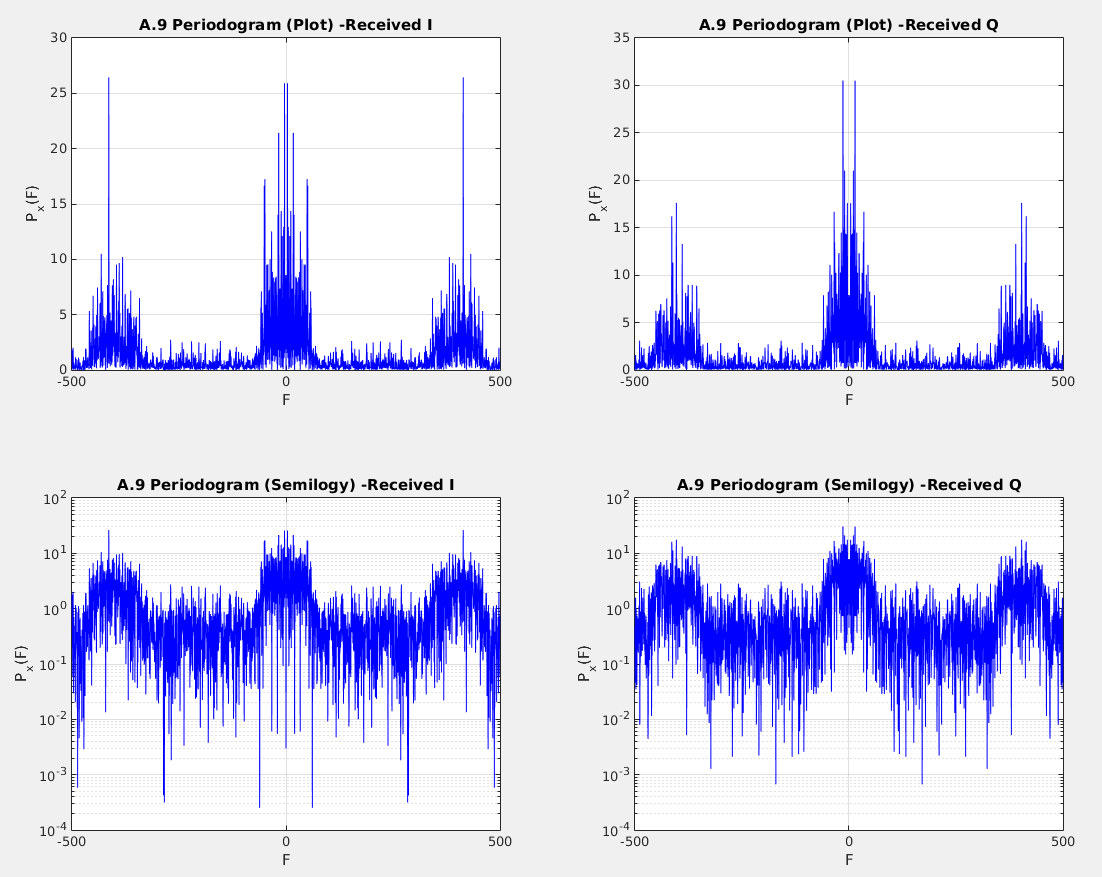
\includegraphics[scale=0.5, width=0.8\textwidth]{img/A9_rec_period.png} \\
        \caption{\texttt{Received signals periodograms}}
    \end{figure}
    
    \newpage \par \noindent
    Σημαντικό σε αυτό το σημείο είναι να παρατηρούμε ότι παρά την αποδιαμόρφωση, συνεχίζουν να υπάρχουν πλευρικοί λοβοί γύρω από την βασική ζώνη στις συχνότητες $2Fo$ και $-2Fo$.
    Θα πρέπει όμως μόλις περάσουν από τα προσαρμοσμένα φίλτρα να εξαφανιστούν και να παραμείνει μόνο το φάσμα βασικής ζώνης.
    
    %-------------------------------------
    %   A.10 subsection
    \subsection*{A.10 $Y_I(t)$ and $Y_Q(t)$}
    Αφού είχαμε αποδιαμορφώσει και διακλαδώσει το σήμα εισόδου περάσαμε τα σήματα αυτά από τα προσα- ρμοσμένα φίλτρα SRRC, ουσιαστικά δηλαδή η συνέλιξη με αυτά.
    Ενώ φτιάξαμε κατάλληλα τον άξονα χρόνου όπως έχουμε ήδη αναφέρει στα προηγούμενα project.
    
    \begin{lstlisting}[caption = {A.10 \texttt{Calculate $Y_I(t)$ and $Y_Q(t)$}}]
% A.10
YI = conv(ch_sig_I,phi_t).*Ts;
YQ = conv(ch_sig_Q,phi_t).*Ts;
t_Xt_Rec = [t_X_mod(1) + t_phi(1) : Ts : t_X_mod(end) + t_phi(end)];
display_waveform_periodogram('A.10', 'Filtered I (Conv)', YI, 'Filtered Q (Conv)', YQ, t_Xt_Rec, t_Xt_Rec, Ts, Nf)
    \end{lstlisting}
    
    \begin{figure}[H]
        \centering
        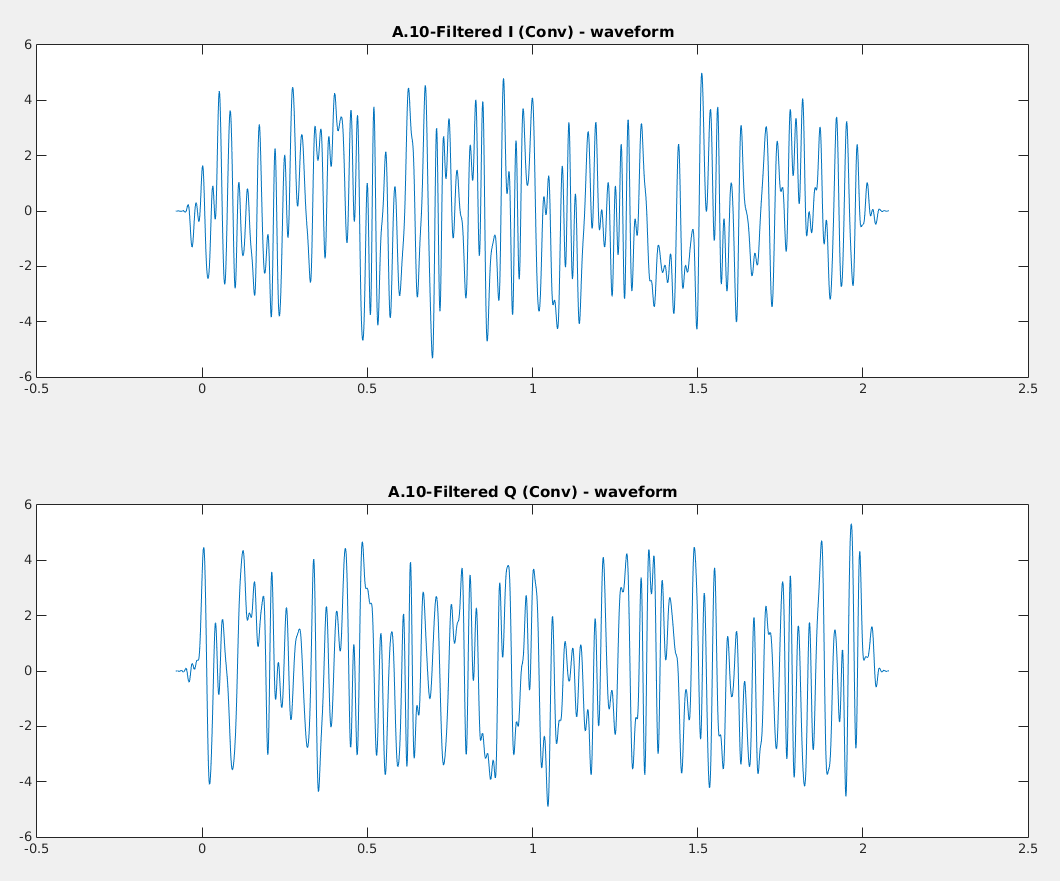
\includegraphics[scale=0.5, width=0.8\textwidth]{img/A10_filt_wave.png} \\
        \caption{\texttt{$Y_I(t)$ and $Y_Q(t)$ waveforms}}
    \end{figure}
    
    \begin{figure}[H]
        \centering
        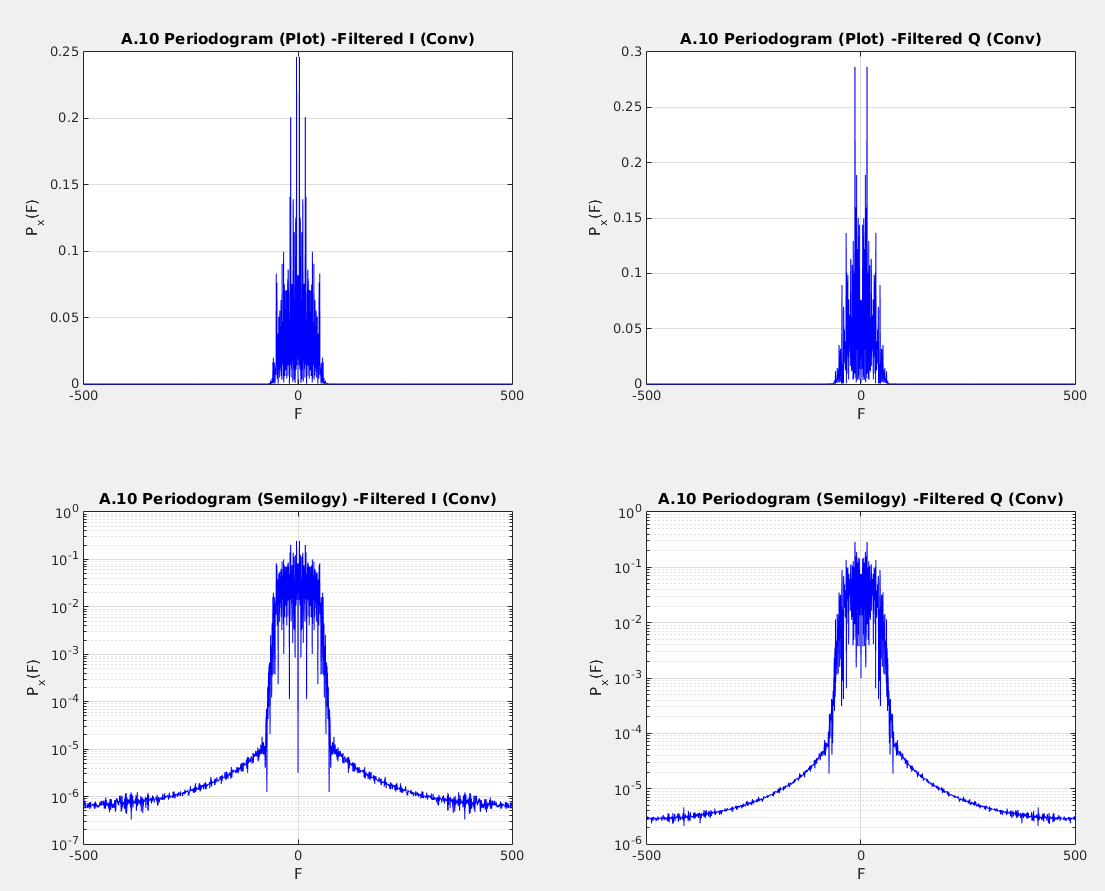
\includegraphics[scale=0.5, width=0.8\textwidth]{img/A10_filt_period.png} \\
        \caption{\texttt{$Y_I(t)$ and $Y_Q(t)$ periodograms}}
    \end{figure}
    
    \par \noindent
    Μπορούμε εύκολα να παρατηρήσουμε σε αυτό το σημείο, ότι έχουν αποκοπεί οι πλευρικοί λοβοί όπως ακριβώς περιμέναμε. Ενώ έχει κρατηθεί μόνο το φάσμα της βασικής ζώνης.
    
    %-------------------------------------
    %   A.11 subsection
    \subsection*{A.11 \{$Y_{I,k}$\} and \{$Y_{Q,k}$\}}
    Έπειτα αυτό που χρειάστηκε να κάνουμε ήταν να δειγματοληπτήσουμε την έξοδο από τα προσαρμοσμένα φίλτρα στις κατάλληλες χρονικές στιγμές και να σχεδιάσουμε την ακολουθία εξόδου χρησιμοποιώντας την εντολή scatterplot. 
    Για την δειγματοληψία έχει ακολουθηθεί ο τρόπος που περιγράφηκε στο φροντιστήριο του μαθήματος και αυτό που ουσιαστικά κάνουμε είναι να αποκόψουμε τα πλευρικά σημεία πριν πάρουμε αυτά που μας ενδιαφέρουν.
    
    \begin{lstlisting}[caption = {A.11 \texttt{Calculate \{$Y_{I,k}$\} and \{$Y_{Q,k}$\}}}]
% A.11
YI_sampled = YI(2*A_s*over+1:over:2*A_s*over+1+N*over); 
YQ_sampled = YQ(2*A_s*over+1:over:2*A_s*over+1+N*over); 
figure() ; scatter(YI_sampled, YQ_sampled); grid on ; title('A.11 Sampled');
    \end{lstlisting}
    
    \begin{figure}[H]
        \centering
        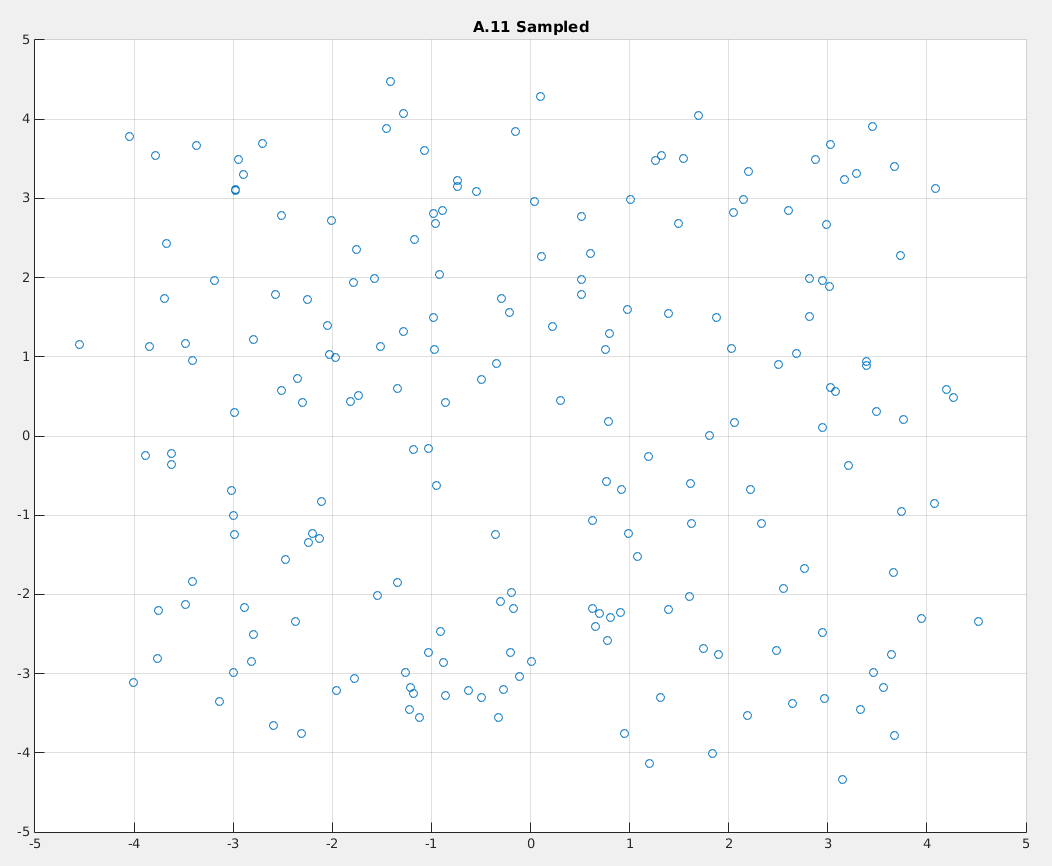
\includegraphics[scale=0.5, width=0.8\textwidth]{img/A11_sampled.png} \\
        \caption{\texttt{Scatterplot \{$Y_{I,k}$\} and \{$Y_{Q,k}$\} for $SNR_{dB}=10$}}
    \end{figure}
    
    \begin{figure}[H]
        \centering
        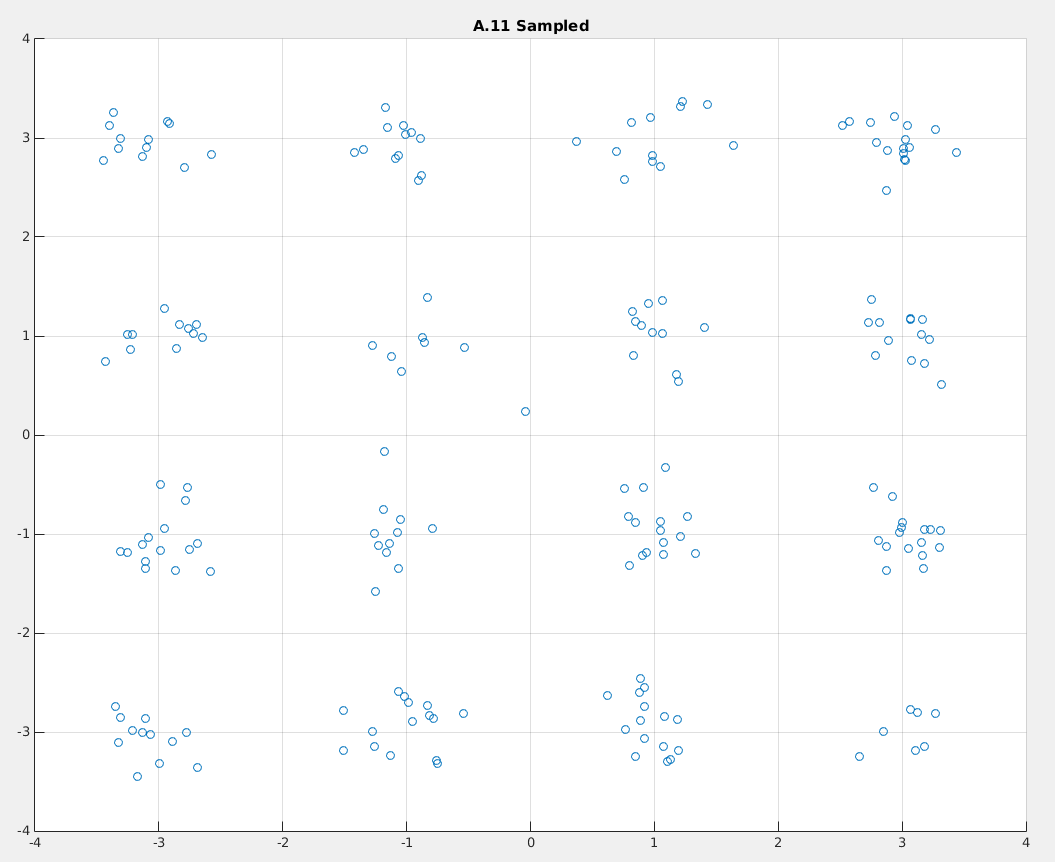
\includegraphics[scale=0.5, width=0.8\textwidth]{img/A11_SNR_20.png} \\
        \caption{\texttt{Scatterplot \{$Y_{I,k}$\} and \{$Y_{Q,k}$\} for $SNR_{dB}=20$}}
    \end{figure}
    
    \par \noindent
    Παραπάνω παρουσιάζεται το scatterplot και για $SNR_{dB}=20$ καθώς είναι πιο κοντά σε αυτό που θα περιμέναμε να δούμε, όμως κρατήθηκε η υλοποίηση για $SNR_{dB}=10$ ώστε να έχουμε περισσότερα σφάλματα και να μπορούμε να δούμε αποτελέσματα και για τα επόμενα ερωτήματα. 
    
    %-------------------------------------
    %   A.12 subsection
    \subsection*{A.12 Estimated symbols}
    Πλέον έπρεπε να δημιουργήσουμε συνάρτηση η οποία θα προέβλεπε πιο σύμβολο έχει σταλθεί χρησι- μοποιώντας τον κανόνα εγγύτερου γείτονα (λόγω των ισοπίθανων συμβόλων) και να αποφασίσει την ακολουθία εισόδου 4-PAM σύμβολο-προς-σύμβολο, ώστε να την εφαρμόσουμε στα δείγματα του inphase και του quadrature.
    Ουσιαστικά πραγματοποιήθηκαν και σε αυτό το σημείο απλές συνθήκες ελέγχου για να επιτευχθεί αυτό.
    
    \begin{lstlisting}[caption = {\texttt{detect\_4\_PAM()}}]
function [est_X] = detect_4_PAM(Y, A)
    est_X=zeros(1,length(Y));
    for i=1:length(Y)
        if(Y(i) > 3*A || (Y(i) > 2*A && Y(i) < 3*A))                        
            est_X(i) = 3*A;                             % -3 | -1 | +1 -> +3
        elseif((Y(i) > 0 && Y(i) < 1*A) || (Y(i) > 1*A && Y(i) < 2*A))      
            est_X(i) = 1*A;                             % -3 | -1 -> +1 <- +3
        elseif((Y(i) < 0 && Y(i) > -1*A) || (Y(i) < -1*A && Y(i) > -2*A))   
            est_X(i) = -1*A;                            % -3 -> -1 <- +1 | +3
        elseif(Y(i) < -3*A || (Y(i) < -2*A && Y(i) > -3*A))                 
            est_X(i) = -3*A;                            % -3 <- -1 | +1 | +3
        end
    end
end
    \end{lstlisting}
    
    \par \noindent
    Ενώ για να την εφαρμόσουμε στα δείγματα που inphase και του quadrature, παρουσιάζεται παρακάτω ο τρόπος κλήσης της.
    
    \begin{lstlisting}[caption = {A.12 \texttt{Setect Symbols}}]
% A.12
YI_est = detect_4_PAM(YI_sampled, A); 
YQ_est = detect_4_PAM(YQ_sampled, A); 
figure() ; scatter(YI_est, YQ_est) ; grid on; title('A.12 Estimations');
    \end{lstlisting}
    
    \begin{figure}[H]
        \centering
        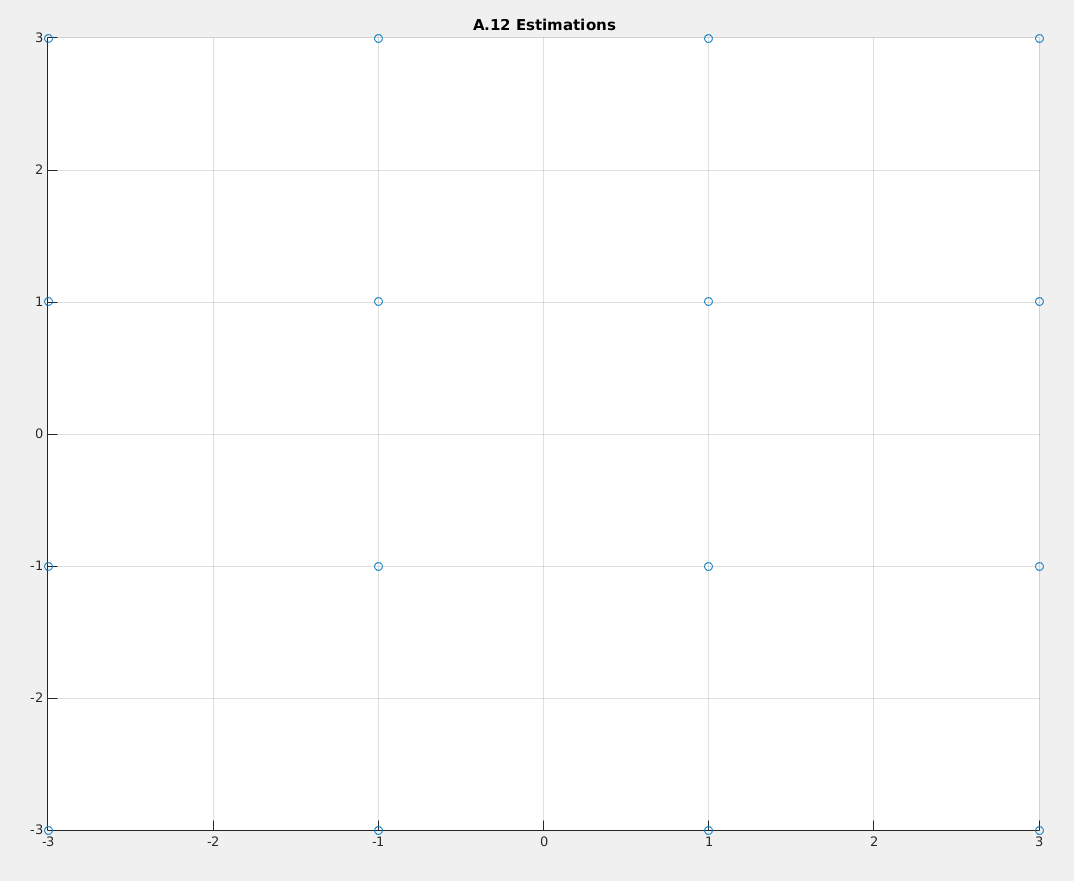
\includegraphics[scale=0.5, width=0.75\textwidth]{img/A12_without_noise.png} \\
        \caption{\texttt{Estimations (Without Noise)}}
    \end{figure}
    
    %-------------------------------------
    %   A.13 subsection
    \subsection*{A.13 Symbols errors}
    Στην συνέχεια χρειάστηκε χρησιμοποιώντας τις ακολουθίες εισόδου και τις αποφάσεις να υπολογιστεί ο αριθμός σφαλμάτων απόφασης συμβόλου για τον αστερισμό 16-QAM.
    Και αυτό έγινε με απλές συνθήκες ελέγχου για ένα προς ένα τα σύμβολα του inphase και του quadrature, με αντίστοιχους μετρητές όταν διαφέρει η είσοδος του καθενός με την ανάλογη απόφαση να αυξάνεται ο εκάστοτε μετρητής. 
    Ενώ στο τέλος έγινε άθροιση των δύο αυτών μετρητών για να υπολογιστεί το σύνολο των λαθών. 
    Όμως προκειμένου να γίνει και οπτική απεικόνιση δημιουργήθηκαν τα arrays Err\_I και Err\_Q τα οποία σε κάθε σημείο που δεν υπάρχει κάποιο λάθος είναι κενό ενώ μόνο στα λάθος σημεία κρατείται η τιμή της λάθος απόφασης \textbf{(εσωτερική στοίχιση επειδή δεν ήταν κάτι που ζητήθηκε)}.
    
    \begin{lstlisting}[caption = {A.13 \texttt{Symbols errors}}]
% A.13
YI_est = YI_est(1:end-1); YQ_est = YQ_est(1:end-1);
I_err = 0;                Err_I=zeros(1,length(YI_est)); Err_I(Err_I==0)=nan;
Q_err = 0;                Err_Q=zeros(1,length(YQ_est)); Err_Q(Err_Q==0)=nan;
for i=1:N
    if(YI_est(i) ~= XI_n(i))
        I_err = I_err + 1;
                          Err_I(i) = YI_est(i);
    end
    if(YQ_est(i) ~= XQ_n(i))
        Q_err = Q_err + 1;
                         Err_Q(i) = YQ_est(i);
    end
end
IQ_err = Q_err + I_err;
disp(['A.13: SER: ', num2str(IQ_err), '/', num2str(N*2)]);
    \end{lstlisting}
    
     %-------------------------------------
    %   A.14 subsection
    \subsection*{A.14 4-PAM to bits}
    Το μόνο που έμενε για την ανάκτηση της πληροφορίες ήταν να δημιουργήσουμε συνάρτηση η οποία θα χρησιμοποιούσε την αντίστροφη απεικόνιση Gray, ώστε να μετατρέψει τα σύμβολα που είχαμε πάρει από τον κανόνα απόφασης σε δυαδική ακολουθία από bits. 
    Για ακόμα μία φορά αυτό επιτεύχθηκε με χρήση απλών συνθηκών, έπρεπε όμως να προσέξουμε ο κανόνας Gray να είναι αντίστοιχος με αυτόν που είχαμε χρησιμοποιήσει στην bits\_to\_4\_PAM().
    
    \begin{lstlisting}[caption = {\texttt{PAM\_4\_to\_bits()}}]
function [est_bit] = PAM_4_to_bits(X, A)
    k=1;
    est_bit=zeros(1,2*length(X));
    for i=1:length(X)
        if(X(i) == 3*A)         % +3 -> 00
            est_bit(k) = 0;
            est_bit(k+1) = 0;
        elseif(X(i) == 1*A)     % +1 -> 01
            est_bit(k) = 0;
            est_bit(k+1) =  1;
        elseif(X(i) == -1*A)    % -1 -> 11
            est_bit(k) = 1;
            est_bit(k+1) = 1;
        elseif(X(i) == -3*A)    % -3 -> 10
            est_bit(k) = 1;
            est_bit(k+1) = 0;
        end
        k=k+2;
    end
end
    \end{lstlisting}
    
    \par \noindent
    Ενώ απλά χρειάστηκε να την καλέσουμε με τον εξής τρόπο.
    
    \begin{lstlisting}[caption = {A.14 \texttt{4-PAM to bits}}]
% A.14
est_bit_XI = PAM_4_to_bits(YI_est, A);
est_bit_XQ = PAM_4_to_bits(YQ_est, A);
est_bit_X = [est_bit_XI est_bit_XQ];
    \end{lstlisting}
    
    %-------------------------------------
    %   A.15 subsection
    \subsection*{A.15 Bits Errors}
    Αφού είχαμε μεταφέρει και ανακτήσει στον δέκτη την πληροφορία που στείλαμε, χρειάστηκε τέλος να υπολογίσουμε τον αριθμό σφαλμάτων σε bit.
    Ο τρόπος με τον οποίο το κάναμε αυτό είναι σε πλήρη αναλογία με αυτόν για τα σύμβολα, ενώ και σε αυτήν την περίπτωση για την οπτική απεικόνιση που υπάρχει στην συνέχεια, υπάρχει σε εσωτερική στοίχιση ο πίνακας Err\_b για τον ίδιο λόγω με τους πίνακες που αναφέρθηκαν νωρίτερα.
    
    \newpage
    \begin{lstlisting}[caption = {A.15 \texttt{Bits errors}}]
% A.15
ber = 0;                Err_b=zeros(1,length(bit_seq)); Err_b(Err_b==0)=nan;
for i=1:length(bit_seq)
    if(bit_seq(i) ~= est_bit_X(i))
        ber = ber + 1;
                        Err_b(i) = bit_seq(i); 
    end
end
disp(['A.15: BER: ', num2str(ber), '/', num2str(N*4)]); 
    \end{lstlisting}
    
    \begin{figure}[H]
        \centering
        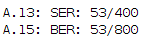
\includegraphics[scale=0.5, width=0.25\textwidth]{img/A13_a15.png} \\
        \caption{\texttt{Matlab output sample for $SNR_{dB}=10$}}
    \end{figure}
    
    \par \noindent
    Στο παρακάτω figure μπορούμε να δούμε (με την χρήση των arrays που αναφέρθηκαν νωρίτερα) σε ποια ακριβώς σύμβολα και bit έχουν υπάρξει σφάλματα κατά την μεταφορά, ώστε να επαληθεύσουμε την ορθότητα των ερωτημάτων. 
    
    \begin{figure}[H]
        \centering
        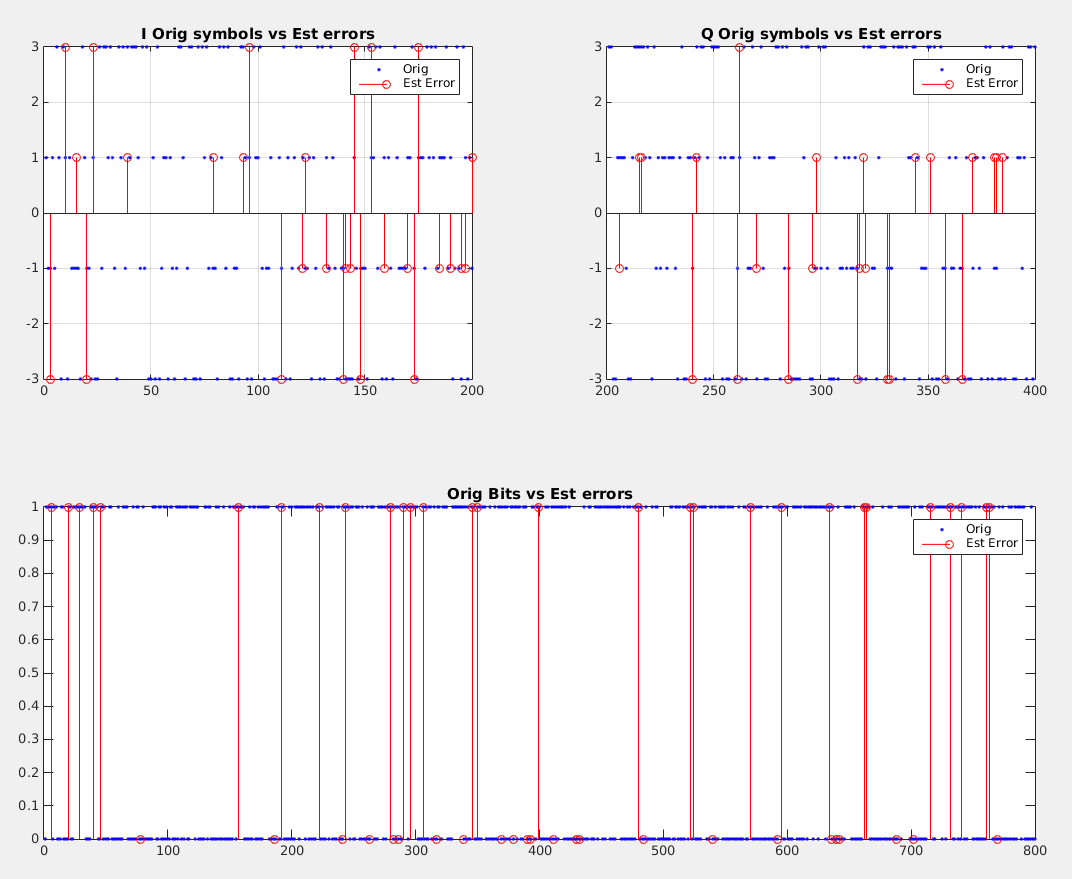
\includegraphics[scale=0.5, width=\textwidth]{img/A13_A15_errors.png} \\
        \caption{\texttt{Error Symbols/Bits Vs Original}}
    \end{figure}
    
    
%---------------------------------------------------------------------------------------------------------------
%
%   Codes
%
%
\newpage

\textbf{\emph{Code:}} \\
\rule{\linewidth}{0.3mm} \\[0.1cm]

    \begin{lstlisting}[caption = {\texttt{bits\_to\_4\_PAM.m}}]
function [ X ] = bits_to_4_PAM(bit_seq, A)
    k=1;
    X=zeros(1,length(bit_seq)/2);
    for i=1:2:length(bit_seq)
        if(bit_seq(i)==0 && bit_seq(i+1)==0)        % 00 -> +3
            X(k) = 3*A;
        elseif(bit_seq(i)==0 && bit_seq(i+1)==1)    % 01 -> +1
            X(k) = 1*A;
        elseif(bit_seq(i)==1 && bit_seq(i+1)==1)    % 11 -> -1
            X(k) = -1*A;
        elseif(bit_seq(i)==1 && bit_seq(i+1)==0)    % 10 -> -3
            X(k) = -3*A;
        end
        k=k+1;
    end
end
    \end{lstlisting}
    %-----------------------------
    \begin{lstlisting}[caption = {\texttt{detect\_4\_PAM.m}}]
function [est_X] = detect_4_PAM(Y, A)
    est_X=zeros(1,length(Y));
    for i=1:length(Y)
        if(Y(i) > 3*A || (Y(i) > 2*A && Y(i) < 3*A))                        % -3 | -1 | +1 -> +3
            est_X(i) = 3*A;
        elseif((Y(i) > 0 && Y(i) < 1*A) || (Y(i) > 1*A && Y(i) < 2*A))      % -3 | -1 -> +1 <- +3
            est_X(i) = 1*A;
        elseif((Y(i) < 0 && Y(i) > -1*A) || (Y(i) < -1*A && Y(i) > -2*A))   % -3 -> -1 <- +1 | +3
            est_X(i) = -1*A;
        elseif(Y(i) < -3*A || (Y(i) < -2*A && Y(i) > -3*A))                 % -3 <- -1 | +1 | +3
            est_X(i) = -3*A;
        end
    end
end
    \end{lstlisting}
    %-----------------------------
     \begin{lstlisting}[caption = {\texttt{fourier\_transform.m}}]
function [X_F, F_X] = fourier_transform(Xt, Ts, Nf)
    Fs = 1/Ts;
    X_F = fftshift(fft(Xt,Nf)*Ts);
    F_X = [-Fs/2 : Fs/Nf : Fs/2-Fs/Nf];
end
    \end{lstlisting}
    %-----------------------------
    \begin{lstlisting}[caption = {\texttt{periodogram.m}}]
function [Px_F, F_Px] = periodogram(Xt, t_Xt, Ts, Nf)
    Ttotal = length(t_Xt)*Ts;
    [X_F, F_Px] = fourier_transform(Xt, Ts, Nf);
    Px_F = (abs(X_F).^2)./Ttotal;
end
    \end{lstlisting}
    
    %-----------------------------
    \begin{lstlisting}[caption = {\texttt{PAM\_4\_to\_bits.m}}]
function [est_bit] = PAM_4_to_bits(X, A)
    k=1;
    est_bit=zeros(1,2*length(X));
    for i=1:length(X)
        if(X(i) == 3*A)         % +3 -> 00
            est_bit(k) = 0;
            est_bit(k+1) = 0;
        elseif(X(i) == 1*A)     % +1 -> 01
            est_bit(k) = 0;
            est_bit(k+1) =  1;
        elseif(X(i) == -1*A)    % -1 -> 11
            est_bit(k) = 1;
            est_bit(k+1) = 1;
        elseif(X(i) == -3*A)    % -3 -> 10
            est_bit(k) = 1;
            est_bit(k+1) = 0;
        end
        k=k+2;
    end
end
    \end{lstlisting}
    %-----------------------------
    \begin{lstlisting}[caption = {\texttt{display\_waveform\_periodogram.m}}]
function [] = display_waveform_periodogram(part, I_text, I_wav, Q_text, Q_wav, t_Xt_I, t_Xt_Q, Ts, Nf)
    % Plot waveforms
    if (~isempty(Q_text)); 
        figure()
        subplot(2,1,1) ; plot(t_Xt_I, I_wav); title(strcat(part, '-', I_text,' - waveform'));
        subplot(2,1,2) ; plot(t_Xt_Q, Q_wav); title(strcat(part, '-', Q_text,' - waveform'));
    else
        figure() ; plot(t_Xt_I, I_wav); title(strcat(part, '-', I_text,' - waveform'));
    end;
    
    %Periodogram
    [Px_F_I, F_I] = periodogram(I_wav, t_Xt_I, Ts, Nf);
    [Px_F_Q, F_Q]= periodogram(Q_wav, t_Xt_Q, Ts, Nf);

    % Plot Periodograms
    if (~isempty(Q_text)); 
        figure()
        subplot(2,2,1); plot(F_I, Px_F_I, 'b') ; grid on; title(strcat(part, ' Periodogram (Plot) -', I_text)) ; xlabel('F') ; ylabel('P_x(F)');
        subplot(2,2,2); plot(F_Q, Px_F_Q, 'b') ; grid on; title(strcat(part, ' Periodogram (Plot) -', Q_text)) ; xlabel('F') ; ylabel('P_x(F)');
        subplot(2,2,3); semilogy(F_I, Px_F_I, 'b') ; grid on; title(strcat(part, ' Periodogram (Semilogy) -', I_text)) ; xlabel('F') ; ylabel('P_x(F)');
        subplot(2,2,4); semilogy(F_Q, Px_F_Q, 'b') ; grid on; title(strcat(part, ' Periodogram (Semilogy) -', Q_text)) ; xlabel('F') ; ylabel('P_x(F)');
    else
        figure()
        subplot(2,1,1); plot(F_I, Px_F_I, 'b') ; grid on; title(strcat(part, ' Periodogram (Plot) -', I_text)) ; xlabel('F') ; ylabel('P_x(F)');
        subplot(2,1,2); semilogy(F_I, Px_F_I, 'b') ; grid on; title(strcat(part, ' Periodogram (Semilogy) -', I_text)) ; xlabel('F') ; ylabel('P_x(F)');
    end;
end
    \end{lstlisting}
       %-----------------------------.
    \begin{lstlisting}[caption = {\texttt{part\_a.m}}]
% ---------------------------------------------------------------------------------
%   Exercise 3, part A
%
%   Authors : Spyridakis Christos
%   Created Date : 15/12/2019
%   Last Updated : 19/12/2019
%
%   Description: 
%               Code created for Exercises of Communication Systems Course
%               in Tecnhical University of Crete
% ---------------------------------------------------------------------------------

clear all ; close all ; clc ;

%% %%%%%%%%%%%%%%%%%%%%%%%%%%%%%%%%%%%%%%%%%%%%%%%%%
% A.1
N = 200;                         % Random bits E.g.
bit_seq = (sign(randn(4*N, 1)) + 1)/2; % 0 1 1 0 . . .

%% %%%%%%%%%%%%%%%%%%%%%%%%%%%%%%%%%%%%%%%%%%%%%%%%%
% A.2
A = 1;                          % Bits to 4 Pam E.g
Xn = bits_to_4_PAM(bit_seq, A);  % +1 -3 -1 -1 +3 . 

%% %%%%%%%%%%%%%%%%%%%%%%%%%%%%%%%%%%%%%%%%%%%%%%%%%
% A.3
XI_n = Xn(1:N);                    % In Phase Symbols
XQ_n = Xn(N+1:2*N);                % Quadrature Symbols

%% %%%%%%%%%%%%%%%%%%%%%%%%%%%%%%%%%%%%%%%%%%%%%%%%%
% A.4
T = 0.01 ; over = 10 ; Ts = T/over ; A_s = 4 ; a = 0.5; 
Nf = 2048 ; Fs = 1/Ts ; F = [-Fs/2 : Fs/Nf : Fs/2-Fs/Nf]; % Frequency vector

% Phi
[phi_t t_phi] = srrc_pulse(T, Ts, A_s, a);

% Create upsampled X_delta signals and using it calculate conv
XI_d = 1/Ts * upsample(XI_n, over) ; XI_t = conv(XI_d, phi_t).*Ts ;
XQ_d = 1/Ts * upsample(XQ_n, over) ; XQ_t = conv(XQ_d, phi_t).*Ts ;
td = [ 0 : Ts : (N*over-1)*Ts ] ; t_Xt = [td(1) + t_phi(1) : Ts : td(end) + t_phi(end)];

% Plot waveforms
figure()
subplot(4,2,1:2) ; stem([1:N*4], bit_seq, 'b') ; title('A.1 Random Bits');
subplot(4,2,3:4) ; stem([1:N*2], Xn, 'r') ; title('A.2 Symbols in 4-PAM');
subplot(4,2,5) ; stem([1:N], XI_n, 'r'); title('A.3 \{X_{I,n}\} - (Xn symbols of In-phase)'); subplot(4,2,6) ; stem([N+1:N*2], XQ_n, 'r'); title('A.3 \{X_{Q,n}\} - (Xn symbols of Quadrature)'); 
subplot(4,2,7) ; plot(t_Xt, XI_t); xlim([-0.1 2.1]) ; ylim([-50 50]) ; title('A.4 X_I (t)'); subplot(4,2,8) ; plot(t_Xt, XQ_t) ; xlim([-0.1 2.1]) ; ylim([-50 50]) ; title('A.4 X_Q (t)');

display_waveform_periodogram('A.4', 'X_i(t)', XI_t, 'X_q(t)', XQ_t, t_Xt, t_Xt, Ts, Nf)

%% %%%%%%%%%%%%%%%%%%%%%%%%%%%%%%%%%%%%%%%%%%%%%%%%%
% A.5
Fo = 200;
XI_mod =  2 * XI_t .* cos(2*pi*Fo*t_Xt);
XQ_mod = -2 * XQ_t .* sin(2*pi*Fo*t_Xt);
display_waveform_periodogram('A.5', 'X_i^{mod}', XI_mod, 'X_q^{mod}', XQ_mod, t_Xt, t_Xt, Ts, Nf)

%% %%%%%%%%%%%%%%%%%%%%%%%%%%%%%%%%%%%%%%%%%%%%%%%%%
% A.6
t_X_mod = t_Xt;
X_mod = XI_mod + XQ_mod;
display_waveform_periodogram('A.6', ' X_{mod} = X_i^{mod} + X_q^{mod} - Plot', X_mod, '', [], t_X_mod, [], Ts, Nf)

%% %%%%%%%%%%%%%%%%%%%%%%%%%%%%%%%%%%%%%%%%%%%%%%%%%
% A.7
% On report

%% %%%%%%%%%%%%%%%%%%%%%%%%%%%%%%%%%%%%%%%%%%%%%%%%%
% A.8
SNR = 10;
var_n = (10*A^2)/(Ts*(10^(SNR/10)));
WGN = sqrt(var_n)*randn(1, length(X_mod));
ch_sig = X_mod + WGN;

%% %%%%%%%%%%%%%%%%%%%%%%%%%%%%%%%%%%%%%%%%%%%%%%%%%
% A.9
ch_sig_I = ch_sig.*cos(2*pi*Fo*t_X_mod);
ch_sig_Q = ch_sig.*(-1*sin(2*pi*Fo*t_X_mod));
display_waveform_periodogram('A.9', 'Received I', ch_sig_I, 'Received Q', ch_sig_Q, t_X_mod, t_X_mod, Ts, Nf)

%% %%%%%%%%%%%%%%%%%%%%%%%%%%%%%%%%%%%%%%%%%%%%%%%%%
% A.10
YI = conv(ch_sig_I,phi_t).*Ts;
YQ = conv(ch_sig_Q,phi_t).*Ts;
t_Xt_Rec = [t_X_mod(1) + t_phi(1) : Ts : t_X_mod(end) + t_phi(end)];
display_waveform_periodogram('A.10', 'Filtered I (Conv)', YI, 'Filtered Q (Conv)', YQ, t_Xt_Rec, t_Xt_Rec, Ts, Nf)

%% %%%%%%%%%%%%%%%%%%%%%%%%%%%%%%%%%%%%%%%%%%%%%%%%%
% A.11
YI_sampled = YI(2*A_s*over+1:over:2*A_s*over+1+N*over); 
YQ_sampled = YQ(2*A_s*over+1:over:2*A_s*over+1+N*over); 
figure() ; scatter(YI_sampled, YQ_sampled); grid on ; title('A.11 Sampled');

%% %%%%%%%%%%%%%%%%%%%%%%%%%%%%%%%%%%%%%%%%%%%%%%%%%
% A.12
YI_est = detect_4_PAM(YI_sampled, A); 
YQ_est = detect_4_PAM(YQ_sampled, A); 
figure() ; scatter(YI_est, YQ_est) ; grid on; title('A.12 Estimations');

%% %%%%%%%%%%%%%%%%%%%%%%%%%%%%%%%%%%%%%%%%%%%%%%%%%
% A.13
YI_est = YI_est(1:end-1); YQ_est = YQ_est(1:end-1);
I_err = 0; Err_I=zeros(1,length(YI_est)); Err_I(Err_I==0)=nan;
Q_err = 0; Err_Q=zeros(1,length(YQ_est)); Err_Q(Err_Q==0)=nan;
for i=1:N
    if(YI_est(i) ~= XI_n(i))
        I_err = I_err + 1;
        Err_I(i) = YI_est(i);
    end
    if(YQ_est(i) ~= XQ_n(i))
        Q_err = Q_err + 1;
        Err_Q(i) = YQ_est(i);
    end
end
IQ_err = Q_err + I_err;
disp(['A.13: SER: ', num2str(IQ_err), '/', num2str(N*2)]);

%% %%%%%%%%%%%%%%%%%%%%%%%%%%%%%%%%%%%%%%%%%%%%%%%%%
% A.14
est_bit_XI = PAM_4_to_bits(YI_est, A);
est_bit_XQ = PAM_4_to_bits(YQ_est, A);
est_bit_X = [est_bit_XI est_bit_XQ];

%% %%%%%%%%%%%%%%%%%%%%%%%%%%%%%%%%%%%%%%%%%%%%%%%%%
% A.15
ber = 0; Err_b=zeros(1,length(bit_seq)); Err_b(Err_b==0)=nan;
for i=1:length(bit_seq)
    if(bit_seq(i) ~= est_bit_X(i))
        ber = ber + 1;
        Err_b(i) = bit_seq(i); 
    end
end
disp(['A.15: BER: ', num2str(ber), '/', num2str(N*4)]); 

    \end{lstlisting}
\end{document}